\chapter{Transfer Function Refinement for Exploring Volume Data \label{transfer_function_refinement}}
Volume visualization is a powerful technique for depicting layered structures in 3D volume data sets. However, it is a major challenge to obtain clear visualizations of a volume with layers clearly revealed.
In particular, the specification of the transfer function is frequently a time-consuming and unintuitive task in volume rendering.
In this chapter, we describe a global optimization and two user-driven refinement methods for modulating transfer functions in order to assist the exploration of volume data.
This optimization is dependent on the distribution of scalar values of the volume data set and is designed to reduce general occlusion and improve the clarity of layers of structures in the resulting images.
The user can explore a volume by interactively specifying different priority intensity ranges and observe which layers of structures are revealed. In addition we show how the technique can be applied for time-varying volume data sets by adaptively refining the transfer function based on the histogram of each time-step. 
Experimental results on various data sets are presented to demonstrate the effectiveness of our method.

%-------------------------------------------------------------------------
\section{Introduction}
%Volume rendering is the process of depicting information within volume data sets, which usually contain complex structures of various materials or dynamic phenomena. The majority of such datasets are discretely sampled along a three-dimensional grid and contain scalar values usually acquired from imaging devices such as CT or MRI machines. In other cases, such as in flow visualization, the datasets are often generated from simulations and may constitute a 3D vector field or multi-variate data of even higher complexity.
%%Volume data is stored as an array of voxels (a three-dimensional extension of pixels), the atomic entities that contain information such as the density or other properties of a discretised position in 3D space.
%Such datasets are ubiquitous in science, medicine and engineering but are difficult to deal with as the data typically does not consist of surfaces and edges, which are the typical primitives of a 3D graphics pipeline. Because of the lack of explicit geometric information, %and limited semantics, 
%it is a major challenge to provide clear visualizations of the structures contained in a volume dataset.

%A crucial step in volume rendering is transfer function specification.
Transfer functions play an essential role in volume rendering.
Through the assignment of visual properties, including color and opacity, to the volume data being visualized,
transfer functions impact the final rendering of the data set and thus affect which structures will be 
visible to the user.
%However, obtaining an effective transfer function is a non-trivial task, which typically involves a significant amount of tweaking of color and opacity.
However obtaining an effective transfer function is a non-trivial task, which often entails time-consuming tweaking until 
a desired aesthetic quality is achieved in the resulting rendering.
%Multi-dimensional transfer functions were developed to distinguish transitions between tissues by utilizing data properties such as gradient and second derivatives.
%%However, high-dimensional transfer functions require high amount of user interaction and the means of interaction is often unintuitive.
%However, the design of high-dimensional transfer functions is usually a very involved and unituitive process for the user.
Although a number of automatic or semi-automatic approaches have been developed, 
transfer function design remains a challenging problem \cite{pfister_transfer_2001} \cite{arens_survey_2010}.
%In interactive volume rendering systems, users can obtain good transfer functions via trial-and-error modification of visualization parameters, but the process often entails time-consuming tweaking until a desired aesthetic quality is achieved in the resulting rendering.
%In addition to the complex structures contained in volume data, users have differing goals or features of interest depending on their specific tasks. Therefore, it is almost impossible to generate a transfer function that would suit all kinds of visualization tasks. Also, different subsets of the data may occlude each other and thus result in ineffective visualization.

For end users, such as physicians, who may not have much experience in volume rendering and transfer function design, 
a user-friendly approach that allows them to intuitively explore volume data sets is very desirable.
%Automatic approaches cannot produce satisfactory results in every case. On the other hand, exploratory approaches with simple and efficient interaction are preferable.
As fully automatic approaches cannot currently guarantee satisfactory results in every case, 
exploratory approaches with simple and efficient interaction are highly desirable.

%Although a variety of multi-dimensional transfer functions have been proposed, they are rarely used in practice, due to their high amount of user interaction, missing precision or unintuitive way of handling it. In practice, the use of simple 1D transfer functions is still dominant \cite{arens_survey_2010}.
%\begin{figure}
%        \centering
%%        \begin{subfigure}[b]{0.3\textwidth}
%        \begin{minipage}{.24\textwidth}
%                \centering
%                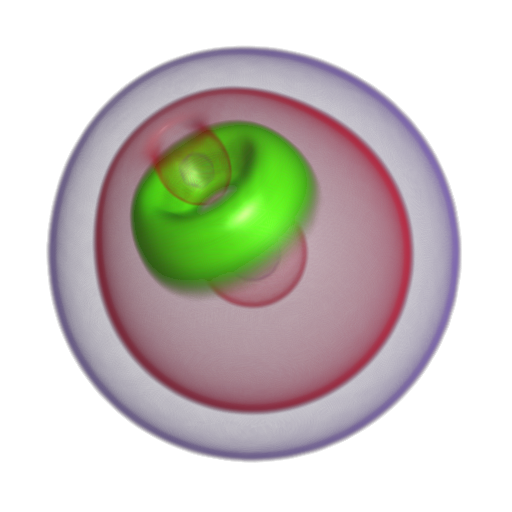
\includegraphics[width=\textwidth]{nucleon.png}
%                \caption{A rendered image with the transfer function in Figure~\ref{fig:tf_nucleon}}
%                \label{fig:nucleon}
%%        \end{subfigure}%
%		\end{minipage}~
%        ~ %add desired spacing between images, e. g. ~, \quad, \qquad etc.
%          %(or a blank line to force the subfigure onto a new line)
%%        \begin{subfigure}[b]{0.3\textwidth}
%        \begin{minipage}{.24\textwidth}
%                \centering
%                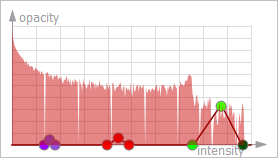
\includegraphics[width=\textwidth]{tf_nucleon.png}
%                \caption{A transfer function with three components. The volume's distribution in logarithmic scale is shown in the background.}
%                \label{fig:tf_nucleon}
%%        \end{subfigure}
%		\end{minipage}
%        \caption{A transfer function and its resulting image of the nucleon data set}\label{fig:multiple_nucleon}
%\end{figure}
%Figure~\ref{fig:tf_nucleon} shows a typical interface for transfer function specification. The control points specify color and opacity for their intensity values. The x-axis is intensity and the y-axis is opacity. Each control point is also assigned a color. The color and opacity of an intensity value is obtained by linear interpolations of the color and opacity of the two adjacent control points. The typical process of transfer function specification involves iterations of assigning colors to control points, moving control points around and then observing the resulting rendered images.
%A rendered image of a nucleon data set is displayed in Figure~\ref{fig:nucleon}. The three components (sets of control points) in Figure~\ref{fig:tf_nucleon} correspond to the three layers in the rendered image.

In this paper, we propose a novel approach to refine the transfer function based on the distribution of the scalar values of the volume data set.
%Our approach provides the ability for users to specify priority intensity ranges in an intuitive way, thus facilitating more interactive exploration of volume data sets.
%This optimization can be done automatically as an initial global optimization with no assumptions of the data set.
Firstly, we propose an automatic step to refine the transfer function that improves the rendering of volume data by reducing overall occlusions with no previous assumptions of the data set. Furthermore, we propose two interactive methods that extend on the optimization technique in order to enhance specific intensity ranges within the data as identified by the user. The process is fast and intuitive and allows the user to provide customized views of the data to aid in visual exploration of the volume data set.

\section{Related Work}
Various strategies have been proposed to simplify transfer function specification \cite{pfister_transfer_2001}.
%Data-centric strategies examine the properties of volume data sets.
Overlapping intensity intervals corresponding to different materials make boundary detection difficult. Classical approaches try to detect boundary information between tissues by introducing derived attributes such as first and second derivatives to isolate materials \cite{kindlmann_semi-automatic_1998} \cite{kniss_multidimensional_2002} \cite{kindlmann_transfer_2002}.
In this case, the transfer functions are extended to multidimensional feature spaces. As a result, the interaction of transfer functions becomes more complex and unintuitive as the dimensionality becomes higher.
%Even two-dimensional transfer functions require a considerable amount of user interaction to find a meaningful shape \cite{arens_survey_2010}.
Even in the case of two-dimensional transfer functions, a considerable amount of user interaction is
required in order to come up with meaningful results \cite{arens_survey_2010}.
%There are other multi-dimensional transfer functions approaches, such as spatialized gradient-based transfer functions \cite{roettger_spatialized_2005}, distance-based transfer functions \cite{tappenbeck_distance-based_2006}, size-based transfer function \cite{correa_size-based_2008}, texture-based transfer functions \cite{caban_texture-based_2008} and curvature based transfer functions \cite{kindlmann_curvature-based_2003}.

Rezk-Salama et al. \cite{rezk-salama_automatic_2000} presented high-level semantics to abstract parametric models of transfer functions in order to automatically assign transfer function templates.
Bruckner and Gr{\"o}ller introduced the concept of style transfer functions \cite{bruckner_style_2007}, which aim to produce more comprehensible images by using transfer functions that map input values to different non-photorealistic rendering styles.
%Another strategy is based on the selection of rendered images. This strategy lets the user select one or more favorite images to guide the further search of transfer functions
%\cite{marks_design_1997}.
Wu and Qu \cite{wu_interactive_2007} developed a method that uses editing operations and stochastic search of the transfer function parameters to maximize the similarity between volume-rendered images given by the user.
%Although researchers have developed a great number of visualization techniques for static volume data, how to effectively explore and understand time-varying volume data remains a challenging problem.
Finding good transfer functions for time-varying volume data is more difficult than for static volume data, as data value ranges and distributions change over time.
Jankun-Kelly and Ma \cite{jankun-kelly_study_2001} examined how to combine transfer functions for different time-steps to generate a coherent transfer function.
Tikhonova et al. \cite{tikhonova_exploratory_2010} presented an explorative approach based on a compact representation of each time step of the dataset in the form of ray attenuation functions. Ray attenuation functions are subsequently used for transfer function generation.

%More recent approaches introduced visibility
%\cite{correa_visibility_2011}
A number of approaches have been proposed to automate the design of transfer functions.
Maciejewski et al. \cite{maciejewski_structuring_2009} described a method to structure attribute space in order to guide users to regions of interest within the transfer function histogram.
Chan et al. \cite{chan_perception-based_2009} developed a system to optimize transparency automatically in volume rendering based on Metelli's episcotister model to improve the perceptual quality of transparent structures.
Correa and Ma \cite{correa_visibility-driven_2009} proposed the visibility histogram to guide the transfer function design. In a later work \cite{correa_visibility_2011}, they generalized the visibility histogram and proposed a semi-automatic method for generating transfer functions by maximizing the visibility of important structures based on the visibility histogram, which represents the contribution of voxels to the resulting image.
Ruiz et al. \cite{ruiz_automatic_2011} also used visibility as a main parameter for the transfer function specification. Their method obtains the opacity transfer function by minimizing the informational divergence between the visibility distribution captured by a set of viewpoints and a target distribution defined by the user. Later, Bramon et al. \cite{bramon_information_2013} extended this approach to deal with multi-modal information.

The approach in this paper is based on our previous work% previous work by Luo and Dingliana
\cite{luo_information-guided_2014} on optimizing transfer functions by minimizing the variance of control point weighting, which is generated from the intensity distribution of the data set. User-selected regions are taken into account, in order to enhance priority intensity ranges of importance to the user in the resulting image, and the approach,  in contrast to others discussed previously, is viewpoint-independent.
In this paper, we extend this further by introducing
%In this paper, we present extensions to this work which introduce 
an intensity-based method to facilitate interactive exploration of volume data sets. In addition, we provide a more generalized approach to the distribution of control points, which in the original paper was limited to simplified tent-shaped distrubtions. Finally we describe how to propagate optimisation of the transfer functions through different time-steps of time-varying data volume sets.
%Recent work on incorporating
%statistical and information metrics into time-varying
%volumetric data includes work by Fang et al. \cite{fang_visualization_2007} on the time
%activity curve, J{\"a}nicke et al. on local statistical complexity
%analysis \cite{janicke_multifield_2007}, and Haidacher et al. \cite{haidacher_information-based_2008} on utilizing information
%theory for fusing traditional transfer function space with
%information enhanced transfer function spaces.

%and measures derived from information theory \cite{haidacher_information-based_2008} 
%\cite{bruckner_isosurface_2010}
%\cite{ruiz_automatic_2011}
%\cite{bramon_information_2013}

%Much of the work in the field of volume visualization has been focused on the synthesis of photorealistic images to assist in the visualization of structures contained in volume data sets.
%However, traditional depictions of the same types of data, such as those found in medical textbooks, deliberately use non-realistic techniques to draw the viewer's attention to important aspects \cite{bruckner_style_2007}. Using abstraction, visual overload is prevented and thus result in a more effective visualization.
%
%Bruckner et al. introduced the concept of style transfer functions \cite{bruckner_style_2007}.
%Techniques from traditional art and illustration are incorporated in the volume rendering process. The goal is to gain clarity compared to photorealism by emphasizing important features, improving data exploration. Less relevant details are omitted and important aspects are highlighted, resulting in more comprehensible images.
%Although researchers have developed a great number of visualization techniques for static volume data, how to effectively explore and understand time-varying volume data remains a challenging problem. Finding good transfer functions for time-varying volume data is more difficult than for static volume data, as data value ranges and distributions change over time.
%%Coherence is an important issue of transfer function design for time-varying volume data.
%Jankun-Kelly and Ma \cite{jankun-kelly_study_2001} examined how to combine transfer functions for different time-steps to generate a coherent transfer function.
%Woodring et al. \cite{woodring_high_2003} considered time-varying volume data as four-dimensional data field and provided a user interface to specify hyperplanes in 4D.
%Woodring and Shen \cite{woodring_chronovolumes_2003} introduced an alternative approach to render multiple time-steps in a sequence with different colors into a single image. This approach provides the context of surrounding time steps but coherence of color among time-steps is hard to maintain.
%Tikhonova et al. \cite{tikhonova_exploratory_2010} presented an explorative approach based on a compact representation of each time step of the dataset in the form of ray attenuation functions. Ray attenuation functions are subsequently used for transfer function generation.
%\cite{maciejewski_structuring_2009}
%\cite{maciejewski_abstracting_2013}
%\cite{mindek_visual_2013}
%\cite{rodriguez_state---art_2014}
%\cite{ip_hierarchical_2012}

%Despite the advances of these methods, transfer function design for volume rendering is still an open research problem.

\section{Background}
\label{sec:background}
%This section describes the background related to our methods.
\subsection{Transfer Function Specification}
%\begin{figure}
%  \centering
%    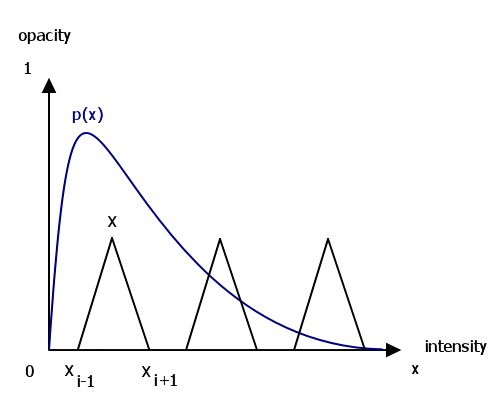
\includegraphics[width=0.6\textwidth]{drawing_distribution.png}
%  \caption{A transfer function with three components which correspond to three intensity intervals}
%  \label{fig:drawing_distribution}
%\end{figure}

%A typical class of 1D (intensity-based) transfer function is based on linear ramps between user-specified control points.

%Volume rendering is used to display a 2D image of a three-dimensional (3D) dataset. It can be seen as a projection of a 3D volumetric dataset into a two-dimensional (2D) image.
%In volume rendering, every volumetric element (voxel) must be mapped to opacity and a color.
%This is done with a transfer function, which can be a simple ramp, a piecewise linear function or an arbitrary table.
%Figure~\ref{fig:konig_mastering_2000} displays four typical shapes used in transfer function design.
%%All the four shapes can reveal structures in volume data sets.
%For volume data sets with complex structures, tent-like shapes are more effective in revealing isosurfaces of structures and seeing through inner structures. Otherwise, the ramp shape and other shapes can also reveal structures effectively.

\begin{table}
\centering
%\begin{minipage}{.5\textwidth}
\normalsize
\begin{tabular}{llll}
\hline
air & fat & soft tissue & bone (cancellous/dense)\\
\hline
-1000 & -100 to -50 & +100 to +300 & +700 to +3000\\
\hline
\end{tabular}
\caption{Hounsfield units of some typical substances \cite{feeman_mathematics_2009}}
\label{table:Hounsfield_unit}
%\end{minipage}
\end{table}

\begin{figure}
\centering

\begin{subfigure}{.16\textwidth}
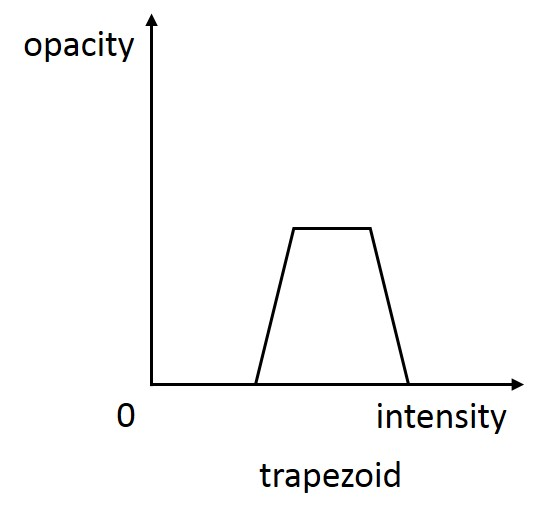
\includegraphics[width=1\textwidth]{konig_mastering_2000-zhou_automatic_2009_a.jpg}
\end{subfigure}
\begin{subfigure}{.16\textwidth}
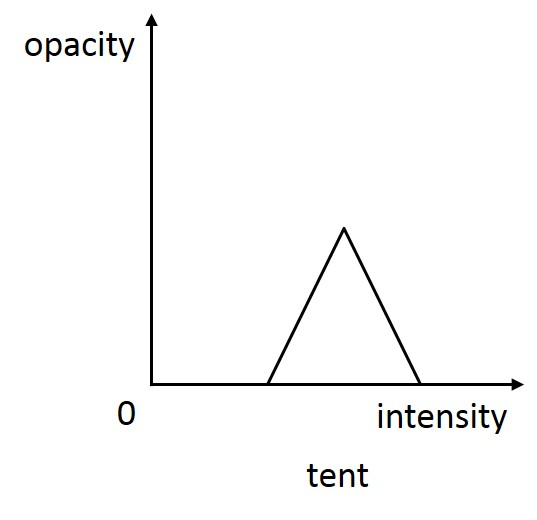
\includegraphics[width=1\textwidth]{konig_mastering_2000-zhou_automatic_2009_b.jpg}
\end{subfigure}
\begin{subfigure}{.16\textwidth}
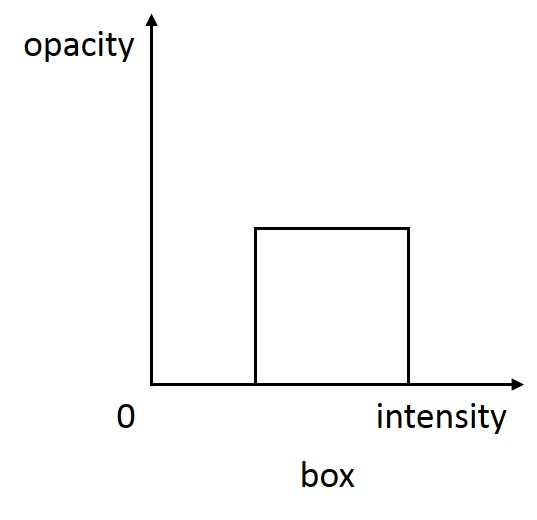
\includegraphics[width=1\textwidth]{konig_mastering_2000-zhou_automatic_2009_c.jpg}
\end{subfigure}
\begin{subfigure}{.16\textwidth}
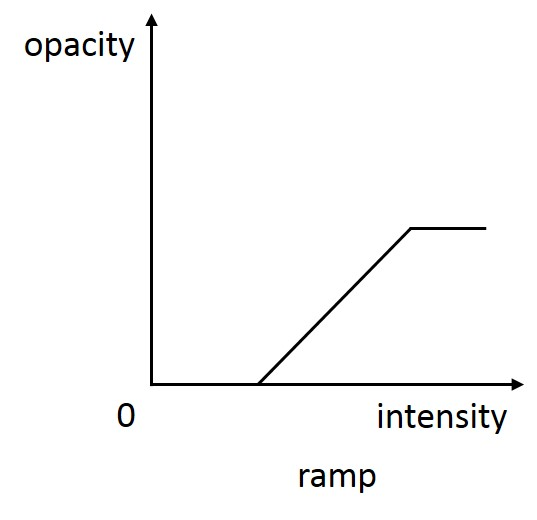
\includegraphics[width=1\textwidth]{konig_mastering_2000-zhou_automatic_2009_d.jpg}
\end{subfigure}
\caption{Typical transfer function shapes \cite{konig_mastering_2000}}
\label{fig:konig_mastering_2000}
\begin{subfigure}{.3\textwidth}
\centering
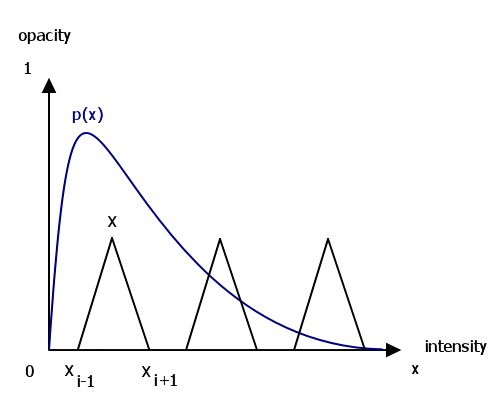
\includegraphics[width=1\textwidth]{drawing_distribution.png}
\end{subfigure}
\caption{A transfer function with tent-like shapes}
\label{fig:drawing_distribution}
\end{figure}

In the specification of a 1D (intensity-based) transfer function, the user essentially assigns a color and/or opacity to a certain point in the histogram of scalar values in the data set. In practice, the user would be presented with an interface that allows them to set up several control points which corresponds to a certain kind of material or structure. The user then defines a mapping from each control points to some visual property (e.g. color) resulting in voxels of the corresponding intensity to be rendered in that color.
Figure~\ref{fig:konig_mastering_2000} displays four typical shapes used in transfer function design.
%All the four shapes can reveal structures in volume data sets.
If a volume data set contains complex structures, tent-like shapes are desirable in revealing isosurfaces of structures and seeing through inner structures. Otherwise, the ramp shape and other shapes can also reveal structures effectively.% \cite{zhou_automatic_2009}

In order to design transfer functions effectively, it is commonly required that users have prior knowledge about which intensity ranges are relevant or which regions should be emphasized in the data. This is especially the case in medical visualization. For instance, in computed tomography (CT) data the intensity ranges are determined by the Hounsfield scale (Table~\ref{table:Hounsfield_unit}). The user may expect the constituent's intensity of CT data to follow the Hounsfield scale and thus set up control points accordingly.
%For instance, they might chose that bone should be mapped on to white and muscle to blue.
%However, small changes made to the opacity of control points may lead to dramatic changes in the rendered images.
%In many cases, minuscule modulation of opacity is required, but this kind of tiny adjustment of control points may be impossible to make accurately through mouse interaction due to limited accuracy of mouse movements.

%Another consideration is that voxels of a particular color can be more visually meaningful to the viewer than voxels of another color.
%An observation by Bordoloi and Shen \cite{bordoloi_view_2005} is that voxels of a particular color can be more visually meaningful to the viewer than voxels of another color.
%For instance, if there are two groups of voxels with different intensity in a scene, if the size of the first group of voxels is considerably less than the second one, then it is possible that the second group of voxels completely occludes the first one.
%Features inside other material are likely to be of far less voxels and are often occluded by the surrounding material.
%Additionally, Gestalt principles \cite{pessoa_finding_1998} suggest that the human mind would extrapolate the larger object (called ground) behind the smaller one (called figure). Thus the first group of voxels should have higher importance than the second one in order to be seen or distinguished.
Another consideration is that interior structures are likely to comprise far fewer voxels and are often occluded by the surrounding material.
Consider the transfer function in Figure~\ref{fig:drawing_distribution}. The user finds three intensity intervals of interest and then sets up three sets of control points in order to visualize these intensity intervals. The opacity of the three peak control points are assigned equally as they are equally important.
However, if the distribution of voxels follows $ p(x) $ (the blue curve), the voxels of the leftmost intensity intervals may completely occlude voxels of the other two intensity intervals in the resulting image.
The global optimization in our approach aims at reducing this kind of occlusion by modulating the opacity of the transfer function based on the distribution of scalar values of the volume data set.
%Figure~\ref{fig:multiple_nucleon} illustrates a transfer function which is more appropriate in this situation.

\subsection{Entropy of Volume Data}
In computer graphics, information-theoretic measures, such as entropy and mutual information, have been applied to solve multiple problems in areas such as view selection \cite{bordoloi_view_2005} 
%\cite{takahashi_feature-driven_2005}
\cite{bramon_information-theoretic_2013}, flow visualization \cite{xu_information-theoretic_2010}, multi-modal visualization \cite{haidacher_information-based_2008} \cite{bramon_information_2013} and transfer function design \cite{bruckner_isosurface_2010} \cite{ip_hierarchical_2012}.
Information theory provides a theoretic framework to measure the information content (or uncertainty) of a random variable represented as a distribution \cite{wang_information_2011}.
Consider a discrete random variable X which has a set of possible values $\{a_{0},a_{1},...,a_{n-1} \}$ with probabilities of occurrence $\{ p_{0},p_{1},...,p_{n-1} \}$, we can measure the uncertainty of the outcome with the entropy H(X), which is defined by
\[  H(X)=-\sum_{x \in X} p(x) \log p(x) \]
where the summation is over the corresponding alphabet and the convention $ 0\log 0=0 $ is taken% \cite{sbert_information_2011}
.
The term $ -\log p(x) $ represents the information content associated with the result x.
If the entire volume data set is treated as a random variable, $ I(a_{x})=-\log p(x) $ represents the information content of a voxel $ a_{x} $ with intensity x, and the entropy gives us the average amount of information of a volume data.
The probability p(x) is defined by
$ p(x)=\frac{n_{x}}{n} $, where $ n_{x} $ is the number of voxels with intensity x and n is the total number of voxels in the volume data.

%In Bordoloi and Shen \cite{bordoloi_view_2005}'s work for view selection of volume rendering, the entire volume data set is treated as a random variable.

%Bordoloi and Shen \cite{bordoloi_view_2005} and Takahashi et al. \cite{takahashi_feature-driven_2005} introduced the entropy to evaluate the quality of a viewpoint.

%In Bordoloi and Shen's work \cite{bordoloi_view_2005}, 

Bordoloi and Shen \cite{bordoloi_view_2005} described a noteworthiness factor to denote the significance of the voxel to the visualization.
The noteworthiness should be high for the voxels which are desired to be seen, and vice versa. The noteworthiness of voxel $ j $ is defined as
$ W_{j}=\alpha_{j}I_{j}=-\alpha_{j}logf_{j} $
, where $ \alpha_{j} $ is the opacity of voxel $ j $ looked up from the transfer function, $ I_{j} $ is the information carried by voxel $ j $, which can be derived from the frequency of its histogram bin $ f_{j} $. -log $ f_{j} $ represents the amount of information associated with voxel $ j $.

\section{Method}
In this section, we present a transfer function refinement approach for modulating the opacity associated with the control points in a transfer function and combine it with user interaction to specify priority areas or intensity values of importance in the resulting image. In previous work \cite{luo_information-guided_2014} we proposed a weighting of control points of transfer functions and an optimization method to minimize the energy function based on this weighting. However, this approach was limited to refining transfer functions with tent-like shapes and processing static volume data sets. 
In this paper we extend this approach with a more general distribution of weightings and energy function, so that it can handle any form of one-dimensional transfer function based on control points. In addition, an interaction widget (as in Figure~\ref{fig:CT-Knee_hue_selection}) is introduced to allow users to explore the data sets by emphasizing certain intensity values and see the optimized output immediately.
%In order to help the user explore the data sets, we combine the automatic optimization process with intuitive user interaction to specify priority areas or intensity values of importance in the resulting image.

In our approach, the user has control of the transfer functions by setting up control points as input for the optimization or tweaking the resulting transfer functions after the optimization. For example, the user can leave out less relevant data ranges by not covering the data ranges with shapes formed by control points (as in Figure~\ref{fig:konig_mastering_2000}). In the case of refining existing transfer functions, users also have the flexibility to refine the input transfer functions partially and keep certain control points constant during the optimization.

\subsection{Weighting of Transfer Function Components}
The goal of our transfer function refinement approach is to balance the opacity settings so that voxels of more significance contribute more and voxels of less significance contribute less to the resulting images.
%An assumption we made in this thesis (Section \ref{motivation}) is that the importance of voxels are associated with their information content. 
%In our approach, the intensity range of the transfer function are normalized to $ [0,1] $.
Given the intensity of the control points $ v_{1},v_{2},...,v_{n} $ of the transfer function $ t $ are $ x_{1},x_{2},...,x_{n} $ and the corresponding opacity are $ \alpha(x_{1}),\alpha(x_{2}),...,\alpha(x_{n}) $. The intensity range of the transfer function is normalized to $ [0,1] $.
For the convenience of discussion, two control points $ v_{0} $ and $ v_{n+1} $ are added to the lower bound and the upper bound respectively, and $ x_{0}=0 $, $ \alpha(x_{0})=0 $, $ x_{n+1}=1 $ and $ \alpha(x_{n+1})=0 $.

Similar to the noteworthiness factor by Bordoloi and Shen \cite{bordoloi_view_2005}, opacity and probability (derived from the intensity histogram) are also used in our weighting.
We define the significance factor of the intensity $ x $ as
\[
s(x)=-\alpha(x)p(x) \log p(x), x \in [0,1]
\]
In the significance factor $ s(x)$, $ p(x) $ is computed from the histogram of the data set, and $ \alpha(x) $ is the opacity function that we want to modulate.
The significance factor should be high for the voxels which are desired to be seen, and vice versa.
Then we define the weight of the $ i $-th edge (the segment between $ v_{i} $ and $ v_{i+1} $) as
\[
e(i)=\int_{x \in [x_{i}, x_{i+1}]} s(x) dx
\]
where $ i \in [0,n]$ and $ x \in [0,1] $.

Hence the energy function with distance factors for the intensity $ x_{0} $ of the transfer function can be defined as the variance of edge weights with the distance factors
\[
E=\sum_{i=0}^{n}(e(i)-\overline{e(i)})^{2}
\]
where $ \overline{e(i)} $ is the mean of edge weights, i.e.
\[
\overline{e(i)}= \frac{\sum_{i=0}^{n}e(i)}{n}
\]
%
%and define the significance factor of the $ i $-th control point as the sum of the weights of its two adjacent edges
%\[
%V(i)=E(i)+E(i-1), i \in [1,n]
%\]
%Then the average significance factor of all the control points is
%\[
%V_{mean}= \frac{\sum_{i=1}^{n}V(i)}{n}
%\]
%Hence the energy function of the transfer function $ t $ can be defined as the variance of the significance factors of control points
%\[
%F(t)=\sum_{i=1}^{n}(V(i)-V_{mean})^{2}
% \]

Consequently, minimizing the energy function is equivalent to flattening the curve of the edge weights.

\subsection{Optimizer}
\label{sec:optimizer}
Constraints are introduced in the search of the parameter space. Control points would only be moved vertically in the transfer function space. In other words, only the opacity associated with control points would be changed. The intensity of control points remains the same. Also, those control points that are marked as constant would not be updated in the optimization process.
These constraints are based on our assumption that the intensity intervals associated with control points are the user's intensity intervals of interest. The user has explored the volume data and set up the transfer function according to his/her needs. Our algorithm aims to help the user reduce occlusion while preserving the user's knowledge or judgements of the data set.

A greedy strategy is employed in our algorithm to minimize the energy function. In each iteration, two operations are performed:
\begin{itemize}
\item Find the edge with the highest weight in the transfer function and reduce the opacity of the control point at its upper end (the vertex with a larger significance factor in the edge's two adjacent vertices).
\item Find the edge with the lowest weight in the transfer function and increase the opacity of the control point at its lower end (the vertex with a smaller significance factor in the edge's two adjacent vertices).
\end{itemize}
%reducing the opacity of the highest control point (with highest significance factor) and increasing the opacity of the lowest control point (with non-zero lowest significance factor).

In our implementation, the optimization ends when it reaches a user-specified iteration count.
The two step sizes in reducing opacity and increasing opacity can both be user-specified, or the first one is user-specified and the second one is computed based on the first one and the ratio of the significance factors of the two chosen control points. The ratio of the two step sizes affects the overall opacity of the resulting image, for instance, the image becomes more opaque or translucent.

\subsection{Distance Factors for Prioritizing Intensity Ranges}
\label{interaction_methods}
The above described optimizer is an approach to balance the global opacity and thus reduce occlusions in the rendered images. In other words, we de-emphasize the most prevalent voxels, which are considered to have a high probability of occluding the rest of the scene and in particular interior structures of the data.

Although global optimization can help deliver images with better overall visibility, small details may be under-enhanced in the global optimization and certain structures in the image may have to be further enhanced for specific purposes. For instance, in an anatomical data set, the global optimization may guarantee that all structures of materials such as skin, bone and flesh are all visible however if the task of the user is specifically to study skin, this may be counter-productive. Thus it is clear that a flexible method guided by user interactions is necessary to achieve various visualization goals. 

In this section, we describe two alternative methods for prioritizing specific intensity ranges in the volume data. The first approach allows the user to interactively select a specific intensity range target that they are interested in and a hue-based distance factor is used to emphasize different intensity ranges based on the target identified by the user. Secondly, we describe a region-based optimization to provide an intuitive method of interaction by choosing regions of interest in the image that are then enhanced in the final rendering.

\subsubsection{Distance Factors for User-Selected Intensity Values}
%In addition, our optimization approach can be applied to explore different intensity ranges in volume data sets.

%We introduce hue-based distance factors to prioritize the specific intensity ranges. 
%Assume each control point is assigned a unique color, we can get the difference of hue in HSV color space between a specific color and the color of a control point.

We introduce distance factors for intensity values to prioritize the specific intensity ranges.
In our implementation, the user can select an intensity value by clicking on a color palette, which uses the same color map in the transfer function.
Assume each control point is assigned a unique intensity value, we can get the difference between a specific intensity value and the intensity value of a control point.

Given the selected intensity $ x_{0} $, we define the distance factor of the $ i $-th control point $ x(i) $ as
\[  D_{h}(i)=|x_{0}-x(i)|, i \in [0,n+1] \]
Linear interpolation is used to obtain the distance factor $ d_{h}(x) $ for the intensity $ x \in [x_{i},x_{i+1}) $

\[ d_{h}(x)=D_{h}(i) + (D_{h}(i+1)-D_{h}(i))\frac{x-x_{i}}{x_{i+1}-x{i}} \]

Therefore, we define the weight of the $ i $-th edge (the segment between $ v_{i} $ and $ v_{i+1} $) with the distance factors as
\[
e_{h}(i)=\int_{x \in [x_{i}, x_{i+1}]} d_{h}(x)s(x) dx
\]
where $ s(x)=-\alpha(x)p(x) \log p(x), x \in [0,1], i \in [0,n]$.

Hence the energy function with distance factors for the intensity $ x_{0} $ of the transfer function can be defined as the variance of edge weights with the distance factors
\[
E_{h}=\sum_{i=0}^{n}(e_{h}(i)-\overline{e_{h}(i)})^{2}
\]
where $ \overline{e_{h}(i)} $ is the mean of edge weights $e_{h}(i)$.
%, i.e.
%\[
%\overline{e_{h}(i)}= \frac{\sum_{i=0}^{n}e_{h}(i)}{n}
%\]

To use the energy function $ E_{h} $ described in this section, we simply need to replace the original energy function with $ E_{h} $ in the previously described optimization algorithm.

%In our approach, the sum of the squared distances $ D_{s} $ between each pixel in the region $ R $ and the $ i $-th control point is used to measure the difference between the region and the control point.
%\[ D_{s}(R,i)=\sum_{r \in R}d(r,c(i))^{2} , i \in [1,n] \]
%We define the difference factor between the region $ R $ and the $ i $-th control point as
%\[ W(R,i)=\frac{D_{s}(R,i)}{\sum_{i=1}^{n}D_{s}(R,i)}, i \in [1,n] \]

%Hence, the distance factor of the $ i $-th control point is
%\[ V_{h}(i)=d_{h}V(i), i \in [1,n] \]
%To use this distance factor with the optimization algorithm described above, we simply need to replace $ V(i) $ with $ V_{h}(i) $ and compute the mean of significance factors accordingly in the energy function.

\subsubsection{Distance Factors for User-Selected Regions}
%In our approach, user manipulations are supported in the transfer function domain. Users can specify opacity values for control points in the transfer function to indicate their importance.
%This user-specified weighting would be taken into account in the optimization process.
In addition to selecting a specific intensity value, the distance factors can also be calculated using a region selected by the user. This region-based selection provides an intuitive method for the user to prioritize specific intensity ranges by selecting a region with the colors of interest in the resulting image.

We introduce region-based distance factors to prioritize the user's region of interest.
%The difference factors indicate the dissimilarity in color between a selected region in the final image and each control point.
%The weighting represents how much the control point contributes to the selected region.
Assume each control point is assigned a unique color, we can get the difference between the color of a pixel in the region (which is selected in image space) and the color of a control point (HSV color space is used in our implementation).

Given the color of the $ i $-th control point is $ c(i) $, the distance between the color of a pixel $ r $ in the region $ R $ and the color of the $ i $-th control point is denoted by $ d(r,c(i)) $. In our approach, the sum of the distances $ D $ between each pixel in the region $ R $ and the $ i $-th control point is used to measure the difference between the region and the control point.
\[ D(R,i)=\sum_{r \in R}d(r,c(i)) , i \in [0,n+1] \]
%We define the distance factor between the region $ R $ and the $ i $-th control point as
Given the selected region $ R $, we define the distance factor of the $ i $-th control point as 
\[ W_{R}(i)=\frac{D(R,i)}{\sum_{i=1}^{n}D(R,i)}, i \in [0,n+1] \]
Linear interpolation is used to obtain the distance factor $ w_{R}(x) $ for the intensity $ x \in [x_{i},x_{i+1}) $

\[ w_{R}(x)=W_{R}(i) + (W_{R}(i+1)-W_{R}(i))\frac{x-x_{i}}{x_{i+1}-x{i}} \]

Therefore, we define the weight of the $ i $-th edge (the segment between $ v_{i} $ and $ v_{i+1} $) with the distance factors as
\[
e_{R}(i)=\int_{x \in [x_{i}, x_{i+1}]} w_{R}(x)s(x) dx
\]
where $ s(x)=-\alpha(x)p(x) \log p(x), x \in [0,1], i \in [0,n]$.

Hence the energy function with distance factors for the region $ R $ of the transfer function can be defined as the variance of edge weights with the distance factors
\[
E_{R}=\sum_{i=0}^{n}(e_{R}(i)-\overline{e_{R}(i)})^{2}
\]
where $ \overline{e_{R}(i)} $ is the mean of edge weights $e_{R}(i)$.
%, i.e.
%\[
%\overline{e_{R}(i)}= \frac{\sum_{i=0}^{n}e_{R}(i)}{n}
%\]

%To use the energy function $ E_{R} $ described in this section, we simply need to replace the original energy function with $ E_{R} $ in the previously described optimization algorithm.

Similarly, in order to use the energy function $ E_{R} $, we need to replace the original energy function with $ E_{R} $ in the previously described optimization algorithm.

%Consequently, the modified significance factor (biased towards the region $ R $) of the $ i $-th control point is
%\[ V_{R}(i)=W_{R}(i)V(i), i \in [1,n] \]
%To use this significance factor with the optimization algorithm described above, we simply need to replace $ V(i) $ with $ V_{R}(i) $ and compute the mean of significance factors accordingly in the energy function.

The distance factors described in this section measure the dissimilarity between a selected region and a control point. Therefore the distance factor would be small if the region has an overall color similar to the color of the control point.
Since we are minimizing the energy function, which is the variance of the edge weights, reducing the distance factors of those control points, which are related to the selected region, will result in their opacity values being increased. As a result, the features (in this case, the intensity intervals) in the selected regions will be enhanced and other features will be de-emphasized in the rendered image.
%The distances in $ D_{s}(R,i) $ are squared, therefore, it results in a weighting which is more biased towards the selected region, compared to the weighting based on non-squared distances.
%It thus leads to further enhanced features with further weaken context in the rendered images.
Since the distance is measured in the color space, the choice of colors for the control points affects the distance measured and thus affects the weighting function.
%For the purpose of generating satisfactory weighting, control points are better to be assigned colors which are dispersed in the color space.

%In addition, other color spaces could be adopted in this approach. The CIE L*u*v* (abbreviated CIELUV) color space, which is a perceptually uniform representation of the color volume, is a potential alternative in terms of measuring difference. Because the CIE L*u*v* color space is perceptually uniform, it has the characteristic that equally distances in the color space correspond to equal perceptual differences, at least for reasonable small distances \cite{ebert_designing_2002}.

\subsection{Adaptive Transfer Functions for Time-Varying Data Sets}
In time-varying data sets, the data value ranges and distributions change among time-steps. A single global transfer function may not be able to adequately catch the details of the data set.
Therefore we exploit the transfer function optimizer (as discussed in Section~\ref{sec:optimizer}) to locally refine the transfer function for each time-step in the data set.
In this case, the user specifies a transfer function for a single time-step of the time-varying data set and using either of the two interaction methods (as discussed in Section~\ref{interaction_methods}) to specify priority intensity ranges.
The transfer function designed for this time-step is taken as an input transfer function and optimised again based on the histogram of the next time-step. Subsequently, the output of next time-step is taken as input of the time-step after it and so forth.

\section{Results and Discussions}
In this section, we present some results to demonstrate the effectiveness of our approach on the CT-knee (379 $ \times $ 229 $ \times $ 305) and VisMale head (128 $ \times $ 256 $ \times $ 256) datasets \cite{website:Roettger_volume_2013} and a time-varying data set of a simulated turbulent vortex flow (128 $\times$ 128 $\times$ 128, 100 time-steps) \cite{ma_high_2000}.
%and four volumes of a horse embryo data set, which are the horse embryo at 35, 37, 39 and 42 days.
Results were generated in our volume rendering system (Figure~\ref{fig:volume_visualizer}) on a computer equipped with an Intel Core i5-2410M CPU, 8GB of RAM and a NVIDIA GeForce GT 540M graphics card.
%Tests were performed on a computer equipped with an Intel Core i5-2410M CPU, 8GB of RAM and a NVIDIA GeForce GT 540M graphics card.

\begin{figure}
    \centering
	\begin{minipage}{.48\textwidth}
        \centering
        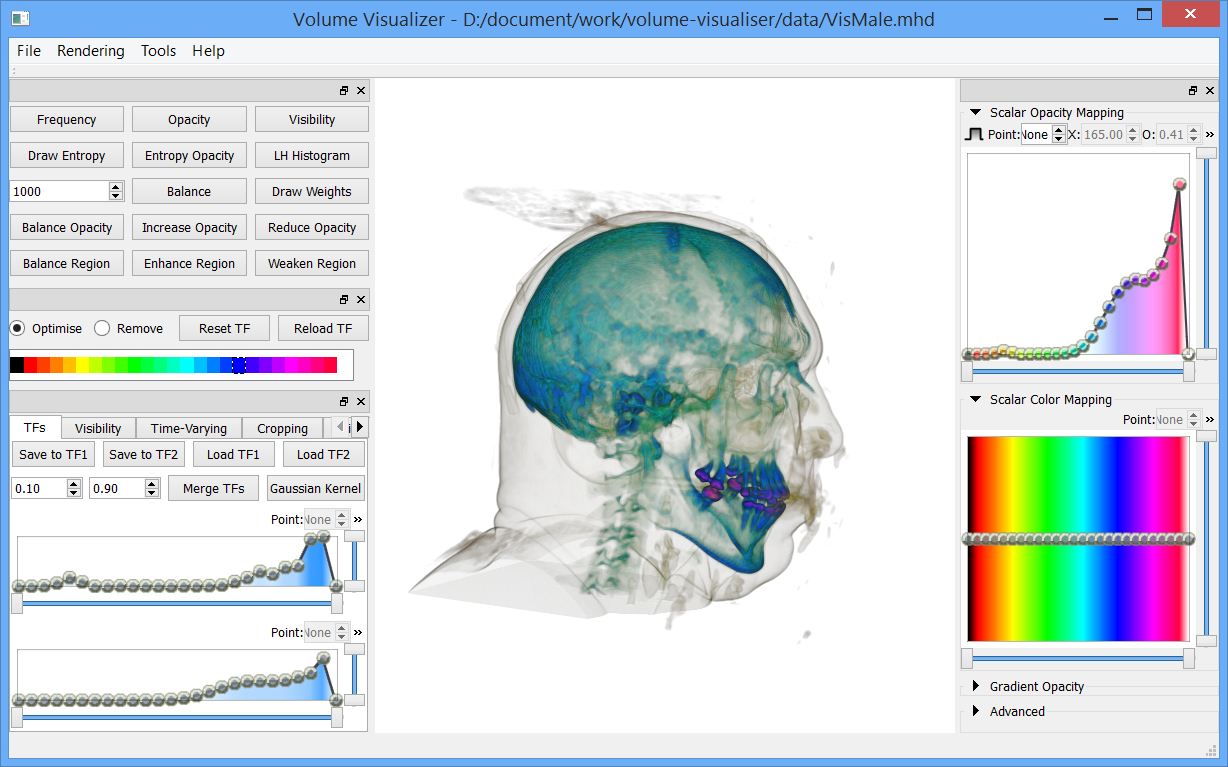
\includegraphics[width=\textwidth]{volume_visualizer.png}
        \caption{A screen shot of our volume rendering system}
        \label{fig:volume_visualizer}
	\end{minipage}
\end{figure}

Automatically generated transfer functions with ramps and tent-like shapes are provided as initial input to the optimizer. Figure~\ref{fig:tf_CT-Knee_spectrum_16_ramp} displays a continuous transfer function. The ramps are formed by a series of control points with corresponding colors from the color map.
Figure~\ref{fig:tf_CT-Knee_spectrum_6} displays a transfer function with several evenly distributed tent-like shapes. Each tent-like shape consists of a peak control point and two bottom control points. The peak control points are movable while the bottom control points are marked as constant to maintain the tent-like shapes.

Note that the transfer functions consisting of equidistant and equal height tent-like shapes (as in Figure~\ref{fig:tf_CT-Knee_spectrum_6}) are just provided as naive examples of user designed transfer functions and used as input to the optimizer. In practice, users would design transfer functions (which consist of ramps, tent-like or other shapes) according to the characteristic of the data sets and the intensity ranges that they are interested in.

%Automatically generated transfer functions with evenly distributed control points are used as the input of the optimization. Two kinds of transfer functions are used in our experiments. One is transfer functions with tent-like shapes (as in Figure~\ref{fig:tf_CT-Knee_spectrum_6} and Figure~\ref{fig:tf_CT-Knee_spectrum_6_balance_1000}), which consist of a number of control point groups (3 control points of the same color) and gaps among the groups. The other is continuous transfer functions (as in Figure~\ref{fig:tf_CT-Knee_spectrum_16_ramp} and Figure~\ref{fig:tf_CT-Knee_spectrum_16_ramp_balance}), which are continuous ramps with control points of different colors.
%Two kinds of transfer functions are used in our experiments.
%One is transfer functions with tent-like shapes (as in Figure~\ref{fig:tf_CT-Knee_spectrum_6} and Figure~\ref{fig:tf_CT-Knee_spectrum_6_balance_1000}), which consist of a number of control point groups (3 control points of the same color) and gaps among the groups. 
%The other is continuous transfer functions (as in Figure~\ref{fig:tf_CT-Knee_spectrum_16_ramp} and Figure~\ref{fig:tf_CT-Knee_spectrum_16_ramp_balance}), which are continuous ramps with control points of different colors.

The initial opacity values of control points will affect the overall opacity level of the resulting image after optimization. Because there are omitted intensity ranges (the gaps) in transfer functions with tent-like shapes, the initial opacity values should be higher in transfer functions with tent-like shapes than in continuous transfer functions.
In transfer functions with tent-like shapes (as discussed in Section~\ref{sec:background}), the opacity of the top control points are set to $ 1/2 $ and the opacity of the bottom control points are set to 0. The bottom control points are fixed to 0 in order to keep the tent-like shapes in the transfer functions. By contrast, all control points in continuous transfer functions are movable vertically except that control points $ v_{0} $ and $ v_{n+1} $ are fixed and serve as the boundary. The opacity of control points are set to $ 1/6 $ in continuous transfer functions.
The color maps used in the transfer functions in our system are evenly sampled from a spectrum (with hue from $ 0^\circ $ to $ 360^\circ $ in HSV color space).
%In the transfer functions, every three adjacent control points with the same color are considered a control point group corresponding to an intensity range.
In the optimization, the two step sizes for reducing opacity and increasing are both set to $ 1/256 $.
%The results below are rendered with Voreen \cite{meyer-spradow_voreen:_2009} after transfer function optimization using our approach.

\subsection{Automatic Transfer Function Refinement}
%\emph{Global Optimisation Results:}
Firstly, we demonstrate the global optimization with continuous transfer functions.
In Figure~\ref{fig:tf_CT-Knee_spectrum_16_ramp}, the CT-Knee data set is rendered with a naive transfer function consisting of 6 tent-like shapes of various colors with equal opacity. Figure~\ref{fig:tf_CT-Knee_spectrum_16_ramp_balance} shows the resulting image rendered with the optimized transfer function.
We tested this specific example as joints are popular regions of interest in medical visualization.
% and a number of researchers have extended volume rendering techniques to examine joints of human body \cite{borland_volumetric_2006}. 
The knee in particular is a commonly studied joint.
In Figure~\ref{fig:tf_CT-Knee_spectrum_16_ramp}, only parts of the skeleton are visible. The rest is occluded by the surrounding material (such as the skin and muscles).
%The knee joint is completely occluded by the surrounding tissues.
After optimization (Figure~\ref{fig:tf_CT-Knee_spectrum_16_ramp_balance}), the surrounding tissues become translucent, hence the skeleton is exposed and the knee joint is visible, while the overall context is preserved. We argue that in the absence of any previous assumptions on what the user is looking for, the global optimization provides a more balanced initial view before deeper exploration of the data.

Although the continuous transfer function is useful in automatic transfer function generation, in typical volume visualization programs, users often prefer much more simplified transfer functions, e.g. a small number of control points such as in transfer functions with tent-like shapes. Figure~\ref{fig:tf_CT-Knee_spectrum_6} is the CT-Knee data set rendered with the transfer function. We show in Figure~\ref{fig:tf_CT-Knee_spectrum_6_balance_1000} that our optimization can also benefit such simpler transfer functions.

In practice we observed that the energy function usually converges to a small but non-zero value. As the number of control points increases, it takes more iterations for the optimization to achieve a stable state - a number of tent-like shapes ranging from 4 to 16 was found to be the most effective.
Our approach is relatively lightweight, e.g. we observed that the optimization finished within one second on the CT-Knee and VisMale data sets with transfer functions consisting of 24 control points and maximum iteration count of 1000.

\begin{figure}
\centering

\begin{subfigure}{0.15\textwidth}
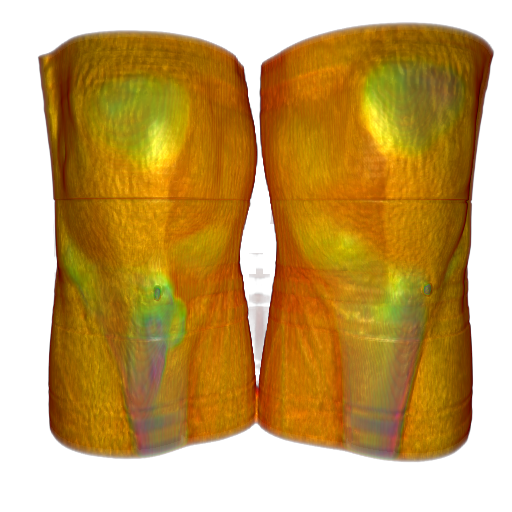
\includegraphics[width=\textwidth]{CT-Knee_spectrum_16_ramp.png}
\caption{~}
\end{subfigure}
\begin{subfigure}{0.15\textwidth}
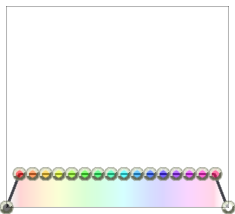
\includegraphics[width=\textwidth]{tf_CT-Knee_spectrum_16_ramp_.png}
\caption{~}
\label{fig:tf_CT-Knee_spectrum_16_ramp_}
\end{subfigure}
\begin{subfigure}{0.15\textwidth}
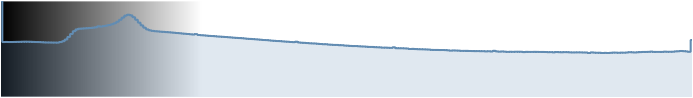
\includegraphics[width=1\textwidth,height=0.75\textwidth]{CT-Knee_histogram.png}
\caption{~}
\label{fig:CT-Knee_histogram}
\end{subfigure}
\caption{Before optimization: CT-Knee with a continuous transfer 
function (a) Preliminary view of data set (b) A continuous transfer 
function with a ramp (c) Histogram of the data set}
\label{fig:tf_CT-Knee_spectrum_16_ramp}

\begin{subfigure}{0.15\textwidth}
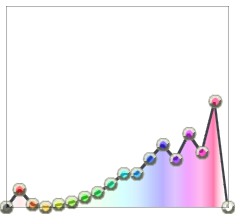
\includegraphics[width=\textwidth]{tf_CT-Knee_spectrum_16_ramp_balance_.png}
\caption{~}
\end{subfigure}
\begin{subfigure}{0.15\textwidth}
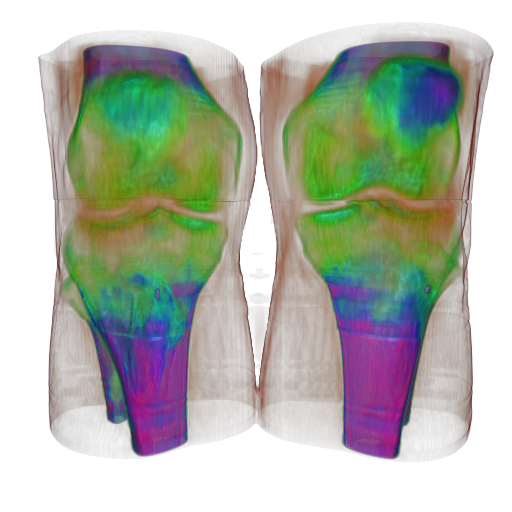
\includegraphics[width=\textwidth]{CT-Knee_spectrum_16_ramp_balance.png}    
\caption{~}
\end{subfigure}
\caption{The transfer function from Figure~\ref{fig:tf_CT-Knee_spectrum_16_ramp} after optimization: (a) Optimized transfer function) (b) Optimized output}
\label{fig:tf_CT-Knee_spectrum_16_ramp_balance}

\end{figure}

\begin{figure}
\centering

\begin{subfigure}{0.15\textwidth}
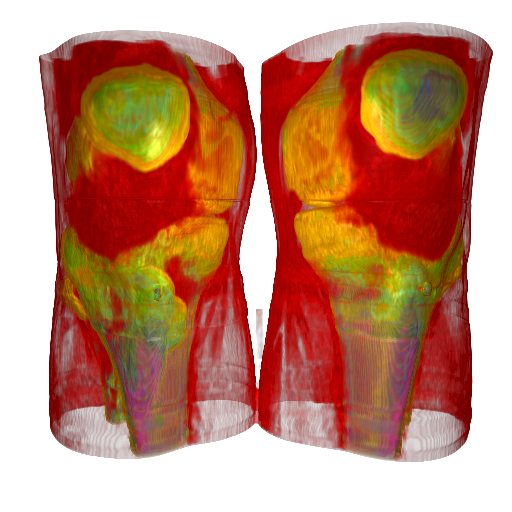
\includegraphics[width=\textwidth]{CT-Knee_spectrum_6_bump.png}
\caption{~}
\end{subfigure}
\begin{subfigure}{0.15\textwidth}
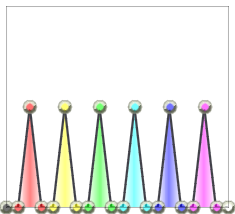
\includegraphics[width=\textwidth]{tf_CT-Knee_spectrum_6_bump_.png}
\caption{~}
\label{fig:tf_CT-Knee_spectrum_6_bump_}
\end{subfigure}
\caption{Before optimization: CT-Knee rendered with a transfer function consisting 
of tent-like shapes (a) Preliminary view of data set (b) A transfer function with 6 tent-like shapes}
\label{fig:tf_CT-Knee_spectrum_6}

\begin{subfigure}{0.15\textwidth}
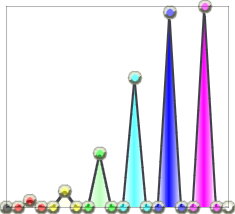
\includegraphics[width=\textwidth]{tf_CT-Knee_spectrum_6_bump_balance_.png}
\caption{~}
\end{subfigure}
\begin{subfigure}{0.15\textwidth}
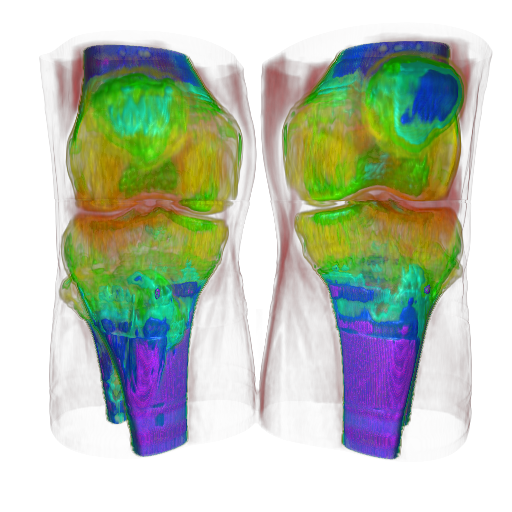
\includegraphics[width=\textwidth]{CT-Knee_spectrum_6_bump_balance.png}
\caption{~}
\end{subfigure}
\caption{The transfer function from Figure~\ref{fig:tf_CT-Knee_spectrum_6} after optimization: (a) Optimized transfer function (b) Optimized output}
\label{fig:tf_CT-Knee_spectrum_6_balance_1000}
\end{figure}

%\paragraph{Distance Factors}
\subsection{Transfer Function Refinement with User-Selected Intensity Values}
%optimising the transfer function to *improve* the exploration of volume data
%In this paragraph, we discuss the results of optimisation with distance factors for user-selected intensity values.
Figure~\ref{fig:CT-Knee_series} shows three images of a CT-Knee data set while different colors are selected for optimization. Since the colors of the transfer function are generated in HSV color space by varying the hue component. The difference of intensity values are mapped to the difference of hue in HSV color space. By clicking on the color palette (Figure~\ref{fig:CT-Knee_hue_selection}), the transfer function is instantly optimized for the corresponding intensity values.

\begin{figure}
    \centering	
	
	\begin{subfigure}{.49\textwidth}
		\centering
		
\includegraphics[width=\textwidth]{CT-Knee_hue_selection_2.png} 
	\end{subfigure}
	
	\begin{subfigure}{.16\textwidth}
	        \centering
	        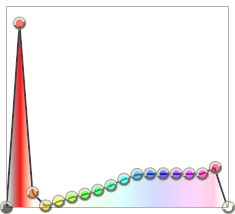
\includegraphics[width=\textwidth]{tf_CT-Knee_hue_00.png}
%	        \caption{}
	        \label{fig:tf_CT-Knee_hue_00.png}
	\end{subfigure}~
	\begin{subfigure}{.16\textwidth}
	        \centering
	        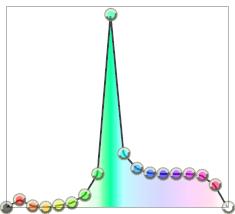
\includegraphics[width=\textwidth]{tf_CT-Knee_hue_07.png}
%	        \caption{}
	        \label{fig:tf_CT-Knee_hue_07.png}
	\end{subfigure}~
	\begin{subfigure}{.16\textwidth}
	        \centering
	        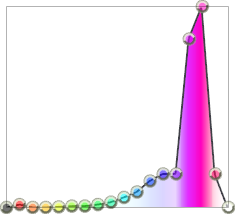
\includegraphics[width=\textwidth]{tf_CT-Knee_hue_14.png}
%	        \caption{}
	        \label{fig:tf_CT-Knee_hue_14.png}
	\end{subfigure}	
	
	\caption{The 3 chosen colors (corresponding to different intensity values) and the transfer functions after optimization for each intensity value. The same transfer function as shown in Figure~\ref{fig:tf_CT-Knee_spectrum_16_ramp} is used as input to the optimizer. Note how the transfer functions are enhanced for the specific intensity ranges as compared to the result of global optimization in Figure~\ref{fig:tf_CT-Knee_spectrum_16_ramp_balance}.}
	\label{fig:CT-Knee_hue_selection}    

	\begin{subfigure}{.16\textwidth}
        \centering
        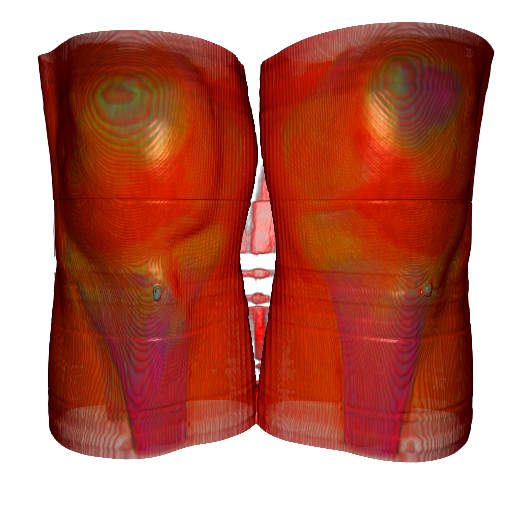
\includegraphics[width=\textwidth]{CT-Knee_hue_00.png}
        \caption{}
        \label{fig:CT-Knee_hue_00.png}
	\end{subfigure}~
	\begin{subfigure}{.16\textwidth}
        \centering
        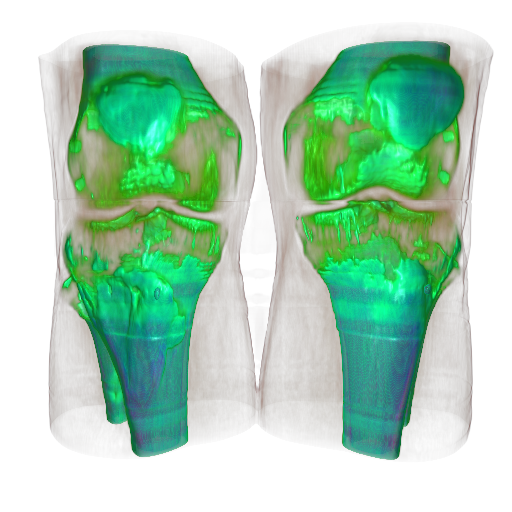
\includegraphics[width=\textwidth]{CT-Knee_hue_07.png}
        \caption{}
        \label{fig:CT-Knee_hue_07.png}
	\end{subfigure}~
	\begin{subfigure}{.16\textwidth}
	        \centering
	        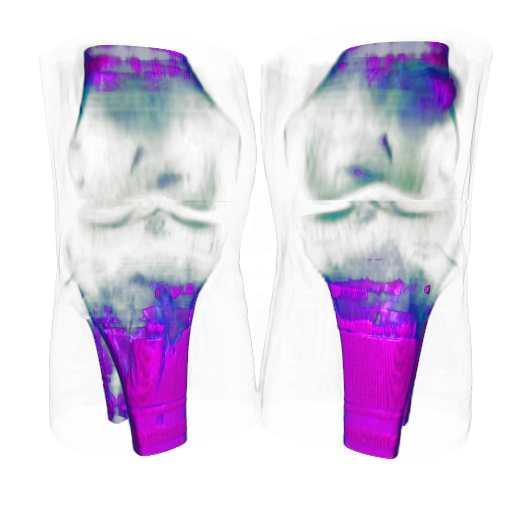
\includegraphics[width=\textwidth]{CT-Knee_hue_14.png}
	        \caption{}
	        \label{fig:CT-Knee_hue_14.png}
	\end{subfigure}
	\caption{The CT-Knee data with transfer functions optimized for the 3 colors in Figure~\ref{fig:CT-Knee_hue_selection}. (a) The materials with intensity values mapped to red are enhanced. Similarly, the materials in green and magenta are enhanced respectively in (b) and (c).}
	\label{fig:CT-Knee_series}	
\end{figure}

\subsection{Transfer Function Refinement with User-Selected Regions}
%\emph{Region-based optimisation}
Figure~\ref{fig:VisMale_spectrum_4_} shows the VisMale data set with a generated transfer function of 4 tent-like shapes. Figure~\ref{fig:VisMale_histogram} shows the intensity histogram of the data set.
%Figure~\ref{fig:VisMale_spectrum_4_balance_1000_} shows the image after optimization.
After the optimization (Figure~\ref{fig:VisMale_spectrum_4_balance_1000_}), the outside of the head is less opaque so the inner structures are revealed to the user. However, the intermediate material (i.e. the skull) also becomes less clear. If the goal is to make the skull more visible, the user could select a region consisting of parts of the skull to generate a weighting and perform further optimization of the transfer function. If the material of interest is occluded by surrounding materials, the user could use an axis-aligned clipping plane in order to accurately select voxels of the skull whilst minimizing the accidental tagging of the surrounding material (Figure~\ref{fig:VisMale_spectrum_4_clipplane_selection}).
%In this step, a clipping plane is used in order to allow the user to more accurately select voxels of the skull whilst minimizing the accidental tagging of the surrounding material.
As shown in Figure~\ref{fig:VisMale_spectrum_4_clipplane_region_1000}, the skull becomes more clear after the region-based optimization.

%A transfer function is manually specified (Figure~\ref{fig:multiple_CT-Knee}) to reveal parts of the bones. The global optimization is performed and more parts of the bones are revealed (Figure~\ref{fig:multiple_CT-Knee_balance}). However, the knee joint is still partial occluded. Then we selected a region of the bones and optimize the transfer function based on the weighting generated for this region. The knee joint is clearly exposed in the resulting images (Figure~\ref{fig:multiple_CT-Knee_region_distance}).
%
%Then we compare the results rendered with two different weighting generated for two selected regions. Figure~\ref{fig:multiple_VisMale7} is a transfer function with even distributed components. Figure~\ref{fig:multiple_VisMale7_balance} shows the result of global optimization. Figure~\ref{fig:multiple_VisMale7_selection} and Figure~\ref{fig:multiple_VisMale7_selection2} show the results of optimization based on two selected regions respectively. From Figure~\ref{fig:VisMale7_region_selection} and Figure~\ref{fig:VisMale7_region_selection} we can see how the two different weighting affects the rendering results.

\begin{figure}
        \centering
	\begin{subfigure}{.16\textwidth}
    \centering
    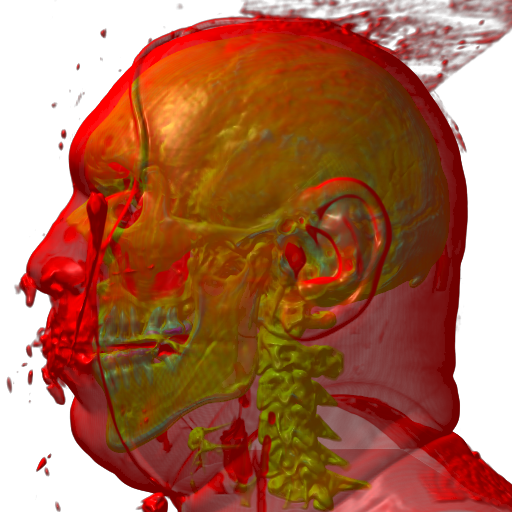
\includegraphics[width=\textwidth]{VisMale_spectrum_4.png}
    \caption{~}
    \label{fig:VisMale_spectrum_4_}
	\end{subfigure}~
	\begin{subfigure}{.16\textwidth}
    \centering
    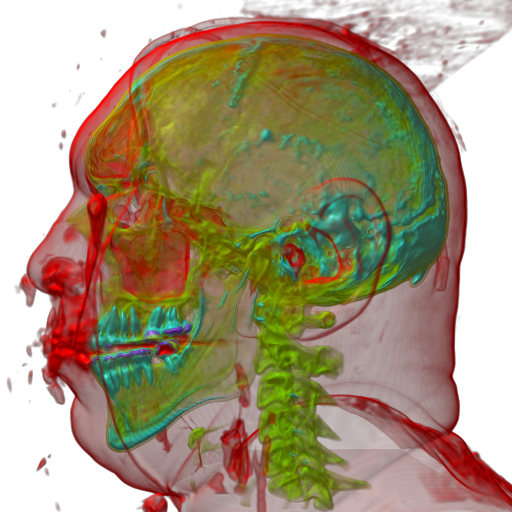
\includegraphics[width=\textwidth]{VisMale_spectrum_4_balance_1000.png}
    \caption{~}
    \label{fig:VisMale_spectrum_4_balance_1000_}
	\end{subfigure}~
	\begin{subfigure}{.16\textwidth}
	\centering
	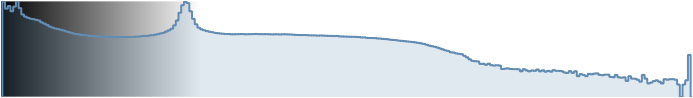
\includegraphics[width=1\textwidth,height=0.75\textwidth]{VisMale_histogram.png}
	\caption{~}
	\label{fig:VisMale_histogram}
	\end{subfigure}
	\begin{subfigure}{.16\textwidth}
	\centering
	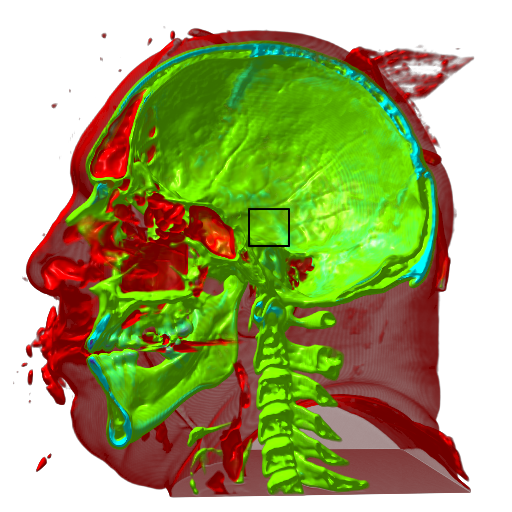
\includegraphics[width=\textwidth]{VisMale_spectrum_4_clipplane_selection.png}
	\caption{~}
	\label{fig:VisMale_spectrum_4_clipplane_selection}
	\end{subfigure}~
	\begin{subfigure}{.16\textwidth}
	\centering
	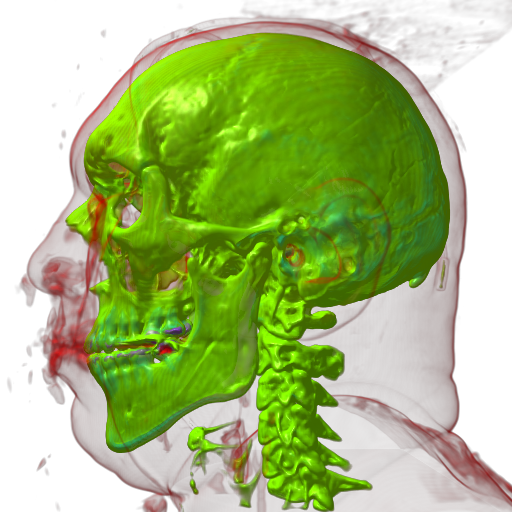
\includegraphics[width=\textwidth]{VisMale_spectrum_4_clipplane_region_1000.png}
	\caption{~}
	\label{fig:VisMale_spectrum_4_clipplane_region_1000}
	\end{subfigure}	
	\caption{(a) Preliminary view of the VisMale data set. (b) Optimized output. (c) Histogram of the data set. (d) The user selects a region on the skull under a clipping plane. (e) Optimized output: skull is enhanced and the outer layer is de-emphasized.}
	\label{fig:multiple_VisMale_spectrum_4_balance_1000}
\end{figure}

%\subsection{Combining Transfer Functions}
%Combine two transfer functions to obtain focus plus context effects.
%
%\begin{figure}
%    \centering	
%	\begin{minipage}{.45\textwidth}
%	        \centering
%	        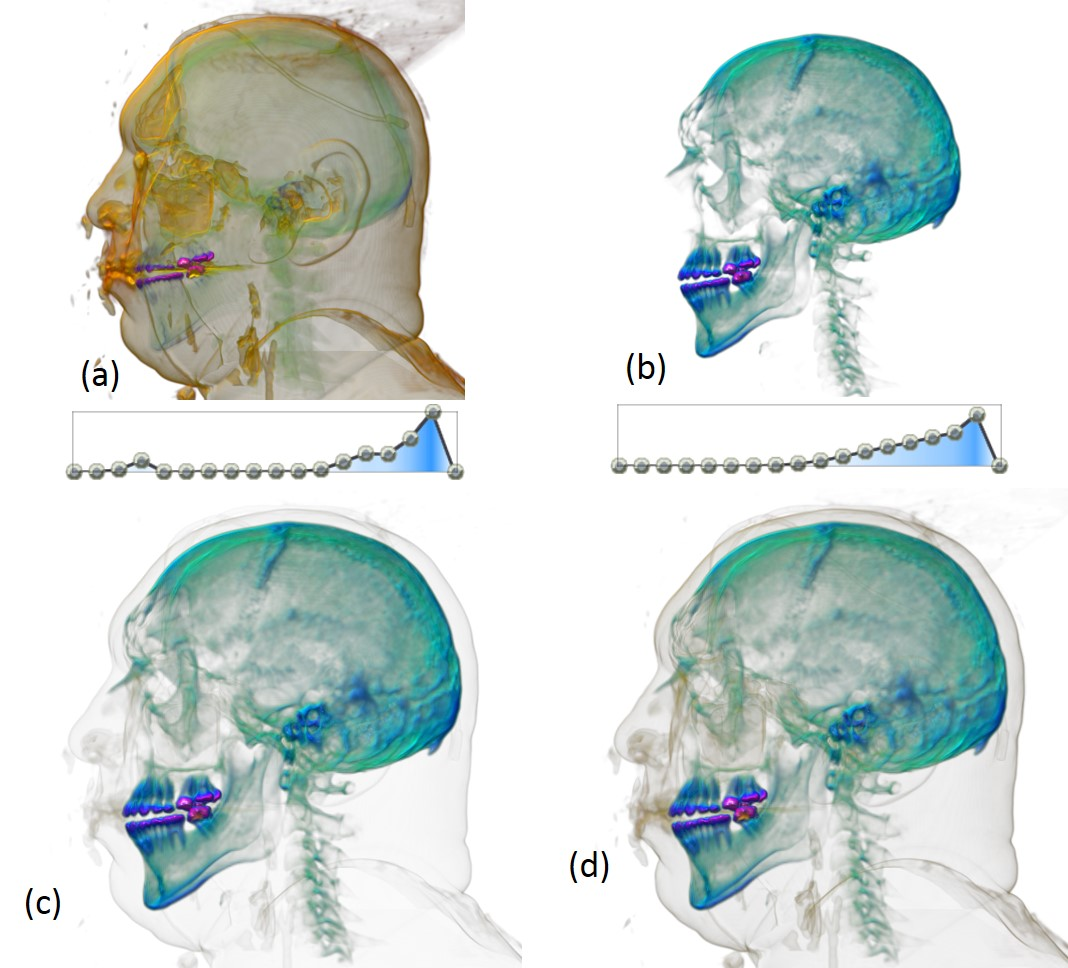
\includegraphics[width=\textwidth]{2_level.jpg}
%%	        \caption{Optimized for magenta}
%%	        \label{fig:2_level}
%	\end{minipage}
%	\caption{2 level}
%	\label{fig:2_level}	
%\end{figure}

\subsection{Adaptive Transfer Functions for Time-Varying Data Sets}
We demonstrate our approach on a turbulent vortex data set \cite{website:Ma_repository_2013}, which consists of 100 time-steps. Our optimizer propagates transfer functions for the time-varying data set in an adaptive way. Specifically, the transfer function of the previous time-step is taken as input to generate the transfer function for the next time-step.
Therefore, the transfer functions are locally optimized for each time-step of the time-varying data set, but as the input transfer function comes from the immediate preceding timestep, the resulting transfer functions also exhibit reasonable temporal coherency assuming the dataset is also coherent.
As the difference of intensity histograms among consecutive time-steps is hard to notice, only the images of the first time-step and a time-step in the middle of the data set are displayed here.
Figure~\ref{fig:vortex_series_time_00} shows three images of the vortex data set at time-step 0 while optimized for the three colors chosen in the color palette in Figure~\ref{fig:vortex_hue_selection}.
Figure~\ref{fig:vortex_series_time_50} displays the vortex data set at time-step 50 with the transfer functions optimized for the three chosen colors.
%Figure~\ref{vortex_time_00_histogram} and Figure~\ref{vortex_time_50_histogram} show the intensity histograms of the two time-steps discussed above.
%In the case that the user does not have much knowledge of a volume data set, our system renders the data set with different ranges being emphasized (see the transfer functions in Figure~\ref{fig:vortex_time_histogram}), in order to provide the user an automatic way to focus their exploration on different parts of the data set.
Figure~\ref{fig:vortex_time_histogram} shows the intensity histograms of the two time-steps discussed above and the corresponding optimized transfer functions for the colors selected in Figure~\ref{fig:vortex_hue_selection}.

\begin{figure}
\centering
	
\begin{subfigure}{.49\textwidth}
\centering

\includegraphics[width=\textwidth]{CT-Knee_hue_selection_2.png}
\end{subfigure}
\caption{The 3 chosen colors (corresponding to different intensity values) for optimization. Note how different parts of the data set are enhanced respectively in Figure~\ref{fig:vortex_series_time_00} and Figure~\ref{fig:vortex_series_time_50}.}
\label{fig:vortex_hue_selection}

\begin{subfigure}{.16\textwidth}
    \centering
    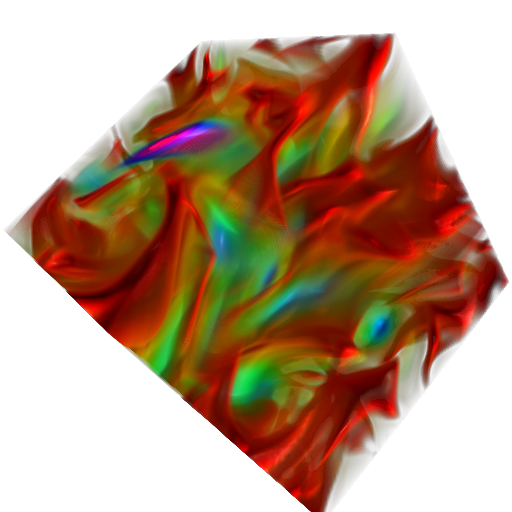
\includegraphics[width=\textwidth]{vortex_time_00_hue_00.png}
    \caption{~}
    \label{fig:vortex_time_00_hue_00}
\end{subfigure}~
\begin{subfigure}{.16\textwidth}
    \centering
    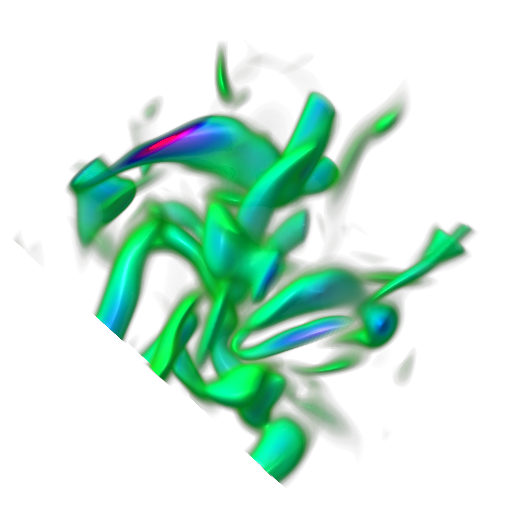
\includegraphics[width=\textwidth]{vortex_time_00_hue_07.png}
    \caption{~}
    \label{fig:vortex_time_00_hue_07}
\end{subfigure}~
\begin{subfigure}{.16\textwidth}
     \centering
     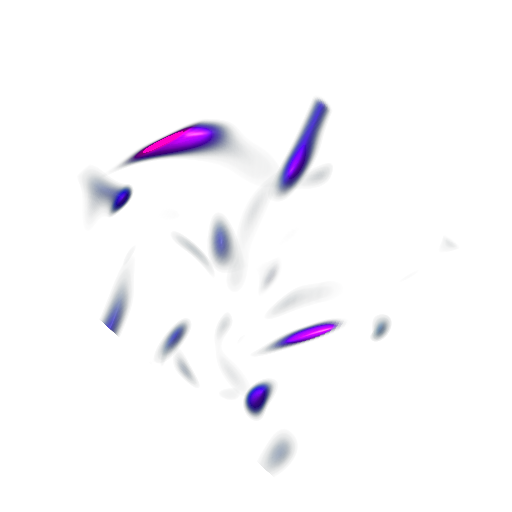
\includegraphics[width=\textwidth]{vortex_time_00_hue_14.png}
     \caption{~}
     \label{fig:vortex_time_00_hue_14}
\end{subfigure}
\caption{The vortex data at time-step 0. (a) The materials with intensity values mapped to red are enhanced. Similarly, the materials in green and magenta are enhanced respectively in (b) and (c).}
\label{fig:vortex_series_time_00}

\begin{subfigure}{.16\textwidth}
    \centering
    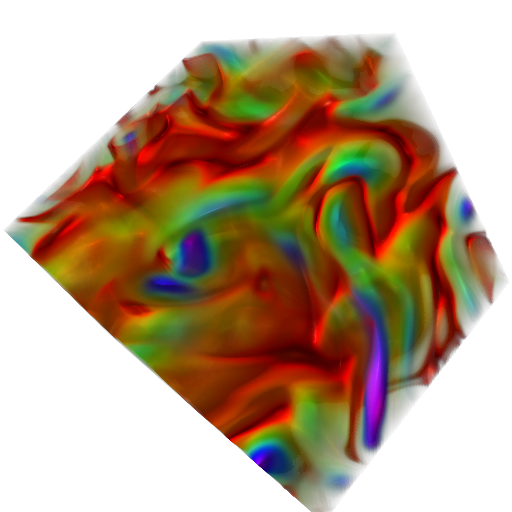
\includegraphics[width=\textwidth]{vortex_time_50_hue_00.png}
        \caption{~}
    \label{fig:vortex_time_50_hue_00}
\end{subfigure}~
\begin{subfigure}{.16\textwidth}
    \centering
    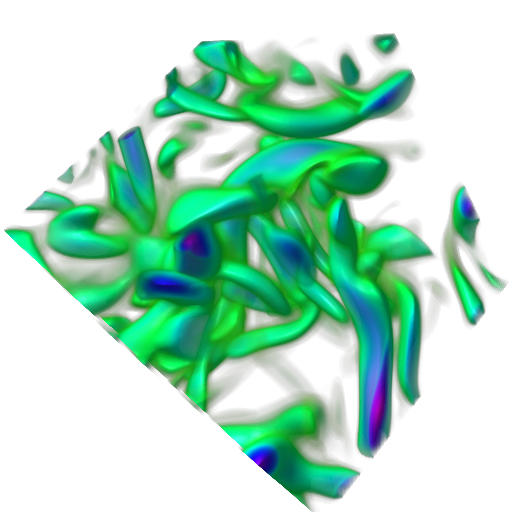
\includegraphics[width=\textwidth]{vortex_time_50_hue_07.png}
        \caption{~}
    \label{fig:vortex_time_50_hue_07}
\end{subfigure}~
\begin{subfigure}{.16\textwidth}
     \centering
     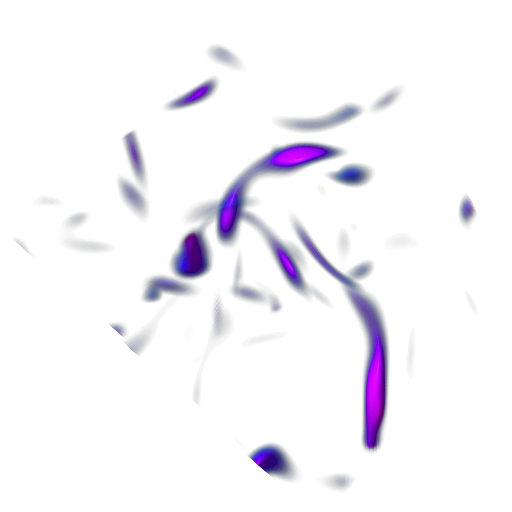
\includegraphics[width=\textwidth]{vortex_time_50_hue_14.png}
	        \caption{~}
     \label{fig:vortex_time_50_hue_14}
\end{subfigure}
\caption{The vortex data at time-step 50. These images show similar results as those for time-step 0, because there are only limited changes among the histograms of different time-steps.}
\label{fig:vortex_series_time_50}
\end{figure}

\begin{figure}
\centering
\begin{subfigure}{.12\textwidth}
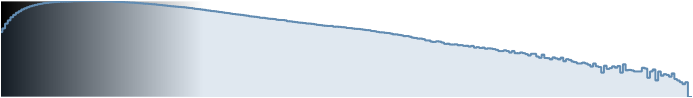
\includegraphics[width=1\textwidth,height=0.75\textwidth]{vortex_time_00_histogram.png}
\caption{~}
\label{vortex_time_00_histogram}
\end{subfigure}~
\begin{subfigure}{.12\textwidth}
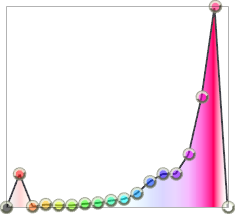
\includegraphics[width=\textwidth]{tf_vortex_time_00_hue_00.png}
\caption{~}
\end{subfigure}~
\begin{subfigure}{.12\textwidth}
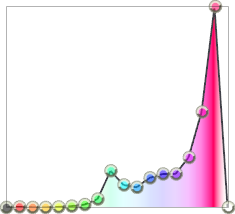
\includegraphics[width=\textwidth]{tf_vortex_time_00_hue_07.png}
\caption{~}
\end{subfigure}~
\begin{subfigure}{.12\textwidth}
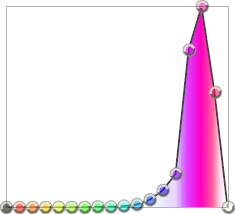
\includegraphics[width=\textwidth]{tf_vortex_time_00_hue_14.png}
\caption{~}
\end{subfigure}

\begin{subfigure}{.12\textwidth}
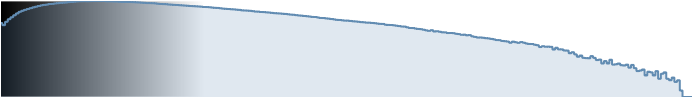
\includegraphics[width=1\textwidth,height=0.75\textwidth]{vortex_time_50_histogram.png}
\caption{~}
\label{vortex_time_50_histogram}
\end{subfigure}~
\begin{subfigure}{.12\textwidth}
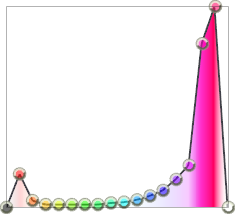
\includegraphics[width=\textwidth]{tf_vortex_time_50_hue_00.png}
\caption{~}
\end{subfigure}~
\begin{subfigure}{.12\textwidth}
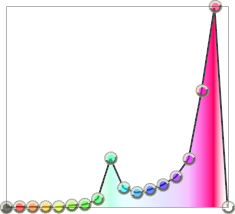
\includegraphics[width=\textwidth]{tf_vortex_time_50_hue_07.png}
\caption{~}
\end{subfigure}~
\begin{subfigure}{.12\textwidth}
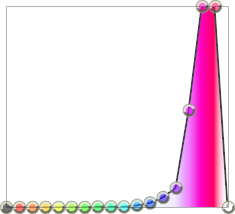
\includegraphics[width=\textwidth]{tf_vortex_time_50_hue_14.png}
\caption{~}
\end{subfigure}
\caption{(a) Histogram of time-step 0.
(b) Transfer function (TF) for Figure~\ref{fig:vortex_time_00_hue_00}.
(c) TF for Figure~\ref{fig:vortex_time_00_hue_07}.
(d) TF for Figure~\ref{fig:vortex_time_00_hue_14}.
(e) Histogram of time-step 50.
(f) TF for Figure~\ref{fig:vortex_time_50_hue_00}.
(g) TF for Figure~\ref{fig:vortex_time_50_hue_07}.
(h) TF for Figure~\ref{fig:vortex_time_50_hue_14}.}
\label{fig:vortex_time_histogram}
\end{figure}

\section{Conclusions}
%The global optimization aims at alleviating occlusion problems in volume rendering. For example, large obstacles, which are common in CT scans of anatomical structures, tend to occlude the rest of structures in the data. If the obstacles has enough opacity, the final image would be dominated by the obstacles. Instead of refining the transfer function based on visibility contribution of voxels \cite{correa_visibility_2011} \cite{ruiz_automatic_2011}, we address this problem by introducing probability distribution from the occurrence of intensity values. Our approach is view-independent and does not required to perform another pass of volume rendering to compute the accumulated opacity for each voxel. Therefore our approach is lightweight and should has better performance compared to approaches which rely on view-dependent visibility distribution.

In this paper, the global optimization aims to alleviate excessive occlusion problems in volume rendering. However, instead of computing the view-dependent visibility of each voxel as is necessitated in other similar approaches \cite{correa_visibility_2011} \cite{ruiz_automatic_2011}, we achieve this by balancing the opacity of voxels based on the distribution of intensity values. Our view-independent approach is relatively lightweight and should have better performance in contrast to other techniques.
%We have implemented an optimization method for improving the exploration of volume data sets.
In addition, we propose two interactive methods that extend on the optimization technique in order to enhance specific intensity ranges within the data as identified by the user.
%The process is fast and intuitive and allows the user to provide customised views of the data to aid in exploration of the volume data set.
This mechanism provides the ability for users to specify priority intensity ranges in an intuitive way, thus facilitating the exploration of both static and time-varying volume data sets.

The main limitation of the approach is that variations to the transfer function are limited to opacity values, which limits, to some degree, the resulting variations in output. The initial choice of intensity ranges, number of control points and color mapping across the histograms can affect the quality of the final output and some prior knowledge of the data sets may be of benefit for optimal results. On the other hand the simple and straightforward techniques presented in this paper should be fully compatible with independent mechanisms for choosing optimal combinations of other visual parameters or indeed if the user wishes to combine these with more manual choices of parameters such as the color map.
%We plan to investigate these areas in our future work.
In addition, the transfer functions in our proposed system are always editable through the user interface. Users may benefit from the flexibility of further tweaking the intensity or opacity of the control points after the application of the automatic optimizations discussed in this paper.

%-------------------------------------------------------------------------
